\cleardoublepage

\section{服务器端程序实现}

整个服务器端程序都采用Rust编程语言\cite{rust}构建。
Rust是一门C或C++编程语言的替代语言,它速度惊人且内存利用率极高。
由于没有运行时和垃圾回收,它能够胜任对性能要求特别高的服务,可以在嵌入式设备上运行,还能轻松和其他语言集成。
它丰富的类型系统和所有权模型保证了内存安全和线程安全,让您在编译期就能够消除各种各样的错误。
另外,它拥有出色的文档、友好的编译器和清晰的错误提示信息,还集成了一流的工具——包管理器和构建工具,
智能地自动补全和类型检验的多编辑器支持,以及自动格式化代码等等。 

\subsection{数据上推流注册模块}
这个模块需要接收客户端上推的原始数据。所使用的协议为WebSocket on HTTPS。
本文选用的Web Server是hyper\cite{hyper},并基于它实现了一个简单的Web框架roa\cite{roa}。

hyper是一个专注正确性和高性能的http库,但过于底层,使用不便。
roa是一个类koajs\cite{koajs}的web框架,灵活而易于拓展。
数据上推流注册模块基于roa框架的HTTPS和WebSocket支持,给每个注册的数据源分配唯一的ID。

数据源注册请求就是一个WebSocket请求:

\begin{lstlisting}[caption={发起数据源注册请求}]
websocket wss://host:port/upstream/
\end{lstlisting}

连接建立之后服务器端给客户端发一个确认包,以告知注册的频道$id$。

\begin{lstlisting}[language=json,firstnumber=1,caption={数据源注册成功}]
{
    "id": 1
}
\end{lstlisting}

我们采用JSON\cite{rfc7159}作为主要的数据传输序列化格式,这段数据告诉客户端注册频道$id$为$1$,数据上推准备已完成。

其逻辑伪代码如下:

\begin{lstlisting}[caption={注册数据源}]
for connection in incomming() {
    id := sources.push(connection)
    connection.send({"id": id})
}
\end{lstlisting}

其中$incomming$函数接受新的请求链接,$sources$数据源频道列表。
原始数据即传感器直接或间接测得的曲率数据,其内容如代码块 ~\ref{lst:raw-data}中所示。

\subsection{曲线重建模块}
图形学上常用的连续化算法(曲线)有贝塞尔(Bezier)曲线、B样条曲线、Catmull Rom样条曲线等;
而统计学上常用线性插值、多项式插值等。图形学连续化的常见目的是得到光滑曲线,而统计学则追求最小偏差。
由于“曲率光滑程度对曲线重建结果的影响”尚无理论研究,也超出了本文的研究范围,故本文采用其中最简便的线性插值法。

线性插值的实现比较简单,伪代码如下:

\begin{lstlisting}[caption={线性插值法}]
raw := raws.first()
for next_raw in raws {
    s := next_raw.s - raw.s
    kka := (next_raw.ka - raw.ka) / s
    kkb := (next_raw.kb - raw.kb) / s
    for i in range(0, s / ds) {
        curvatures.push({"ka": raw.ka + kka * i, "kb": raw.kb + kkb * i})
    }
    raw = next_raw
}
\end{lstlisting}

其中$raws$为一组原始数据,其每个成员数据都包含一个测量点的弧长曲率数据;
$ds$为采用的插值步长;
$curvatures$为插值后的曲率数据。
得到连续化后的曲率数据 $curvatures$ 如代码块 ~\ref{lst:curvature-vec}中所示。

曲线重建算法需要的运算(如加减乘除、三角函数、平方开方和矩阵运算)Rust语言库均有提供。核心逻辑伪代码如下:

\begin{lstlisting}[caption={曲线重建}]
for ka, kb in curvatures {
    k := (ka.powi(2) + kb.powi(2)).sqrt() // composite curvature
    theta := k * ds
    cos_alpha := ka / k
    sin_alpha := kb / k
    cos_theta := theta.cos()
    sin_theta := theta.sin()
    da := cos_alpha * (1. - cos_theta) / k
    db := sin_alpha * (1. - cos_theta) / k
    dc := sin_theta / k

    // get generalized inverse of ti; then dot product relative coordinate
    ti = ri.pseudo_inverse(0.000000001)? * Vector3::new(da, db, dc)
    // ai + ti, to get absolute coordinate of current point
    ai += ti

    column := ai.column(0)
    // push absolute coordinate of current point
    points.push(Point {
        x: column[0],
        y: column[1],
        z: column[2],
    })

    // get next rotation matrix
    ri = Matrix3::new(
        cos_alpha, -sin_alpha, 0.,
        sin_alpha, cos_alpha, 0.,
        0., 0., 1.,
    ) * Matrix3::new(
        cos_theta, 0., sin_theta,
        0., 1., 0.,
        -sin_theta, 0., cos_theta,
    ) * Matrix3::new(
        cos_alpha, sin_alpha, 0.,
        -sin_alpha, cos_alpha, 0.,
        0., 0., 1.,
    ) * ri
}
\end{lstlisting}

重建出的坐标点数据如代码块~\ref{lst:positions}所示。

\subsection{数据下推流模块}

重建数据订阅请求同样是一个WebSocket请求:

\begin{lstlisting}[caption={重建数据订阅}]
websocket wss://host:port/downstream/:id
\end{lstlisting}

其中的$:id$为频道$id$,在上推数据源注册时获得。
重建数据下推流中的一份数据样例如代码块 ~\ref{lst:positions}所示。
其逻辑伪代码如下:

\begin{lstlisting}[caption={订阅数据源}]
for id, connection in incomming() {
    source := sources.get(id)
    connection.subscribe(source)
}
\end{lstlisting}

\subsection{重建效果与误差分析}

本节主要内容是重建算法的效果展示与误差分析。
为了方便画图和分析,所用曲线为二维标准余弦曲线。

\subsubsection{结果与误差}

图 ~\ref{fig:cos} 为标准余弦曲线与插值步长为$0.01$时的重建结果对比图。
图 ~\ref{fig:cos-error} 展示了根据横坐标$x$变化的重建误差,误差定义为两曲线$y$轴坐标之差的绝对值。

由图可知标准余弦曲线一个周期内的重建误差都在$0.05$以内。


\begin{figure}[H]
\centering
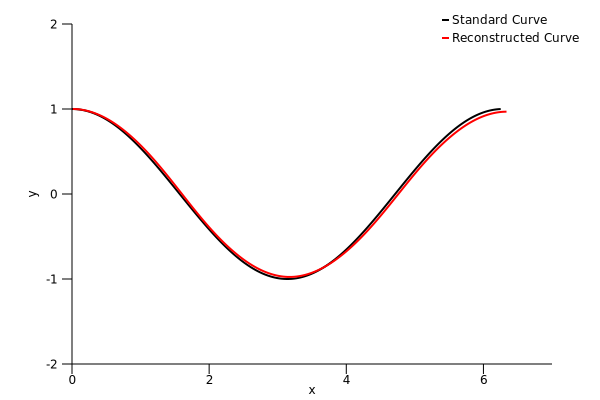
\includegraphics{cos.pdf}
\caption{余弦曲线重建结果}
\label{fig:cos}
\end{figure}

\begin{figure}[H]
\centering
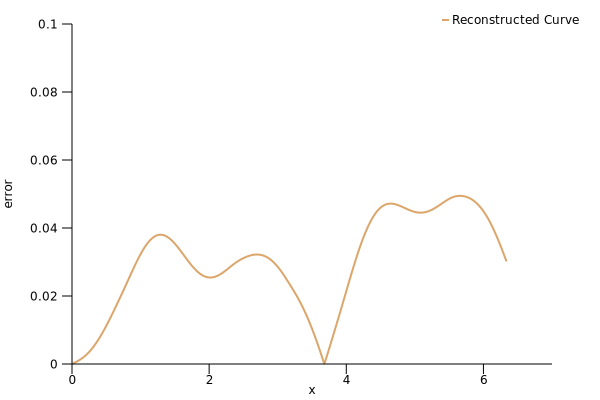
\includegraphics{cos-error.pdf}
\caption{余弦曲线重建误差}
\label{fig:cos-error}
\end{figure}

\subsubsection{不同步长下的误差}

图 ~\ref{fig:cos-diff-step} 为标准余弦曲线与不同插值步长的重建结果对比图。
图 ~\ref{fig:cos-diff-step-error} 展示了横坐标$x$变化下不同插值步长的重建误差。

可知步长越小重建误差越小,但步长从$0.01$减少到$0.001$带来的准确性提升并不是很明显,却增加了十倍的计算负担,
故可认为$0.01$为最适插值步长。

\begin{figure}[H]
\centering
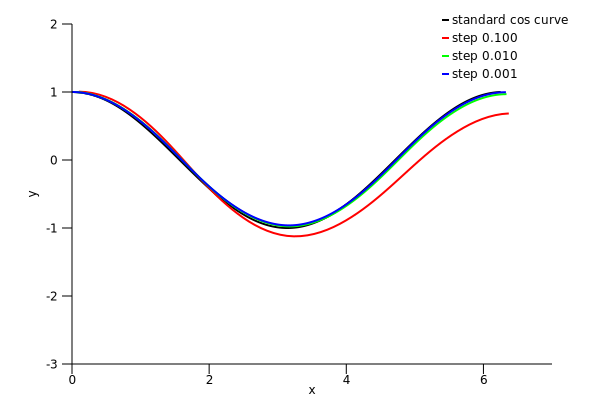
\includegraphics{cos-diff-step.pdf}
\caption{不同步长下的重建结果}
\label{fig:cos-diff-step}
\end{figure}

\begin{figure}[H]
\centering
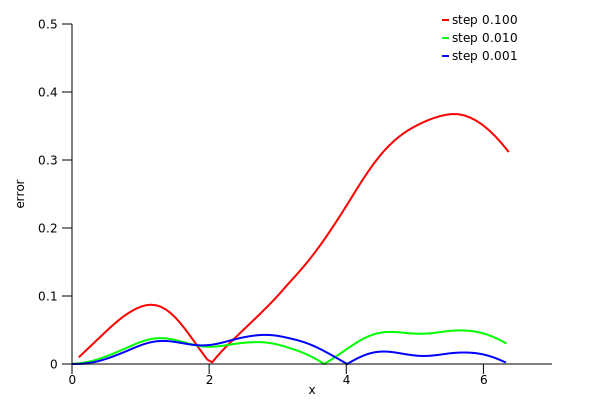
\includegraphics{cos-diff-step-error.pdf}
\caption{不同步长下的重建误差}
\label{fig:cos-diff-step-error}
\end{figure}

\subsubsection{误差传递}

图 ~\ref{fig:cos-single-error-view} 为$x = \frac{\pi}{4}$处加入不同曲率数据误差的重建结果,曲率误差的定义为原始曲率的倍数。
图 ~\ref{fig:cos-single-error} 展示了横坐标$x$变化下加入单点曲率误差的的重建误差传递。

可知单点曲率误差越大重建误差也越大,
且每增加$0.1$倍的曲率误差对重建结果的影响都是巨大的,故原始曲率数据的准确性十分重要。

\begin{figure}[H]
\centering
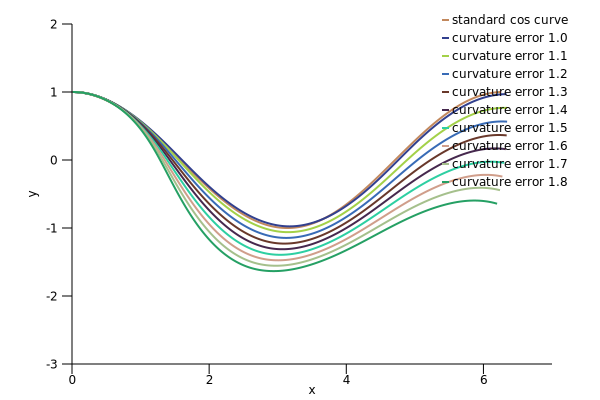
\includegraphics{cos-single-error-view.pdf}
\caption{加入单点误差的重建结果}
\label{fig:cos-single-error-view}
\end{figure}

\begin{figure}[H]
\centering
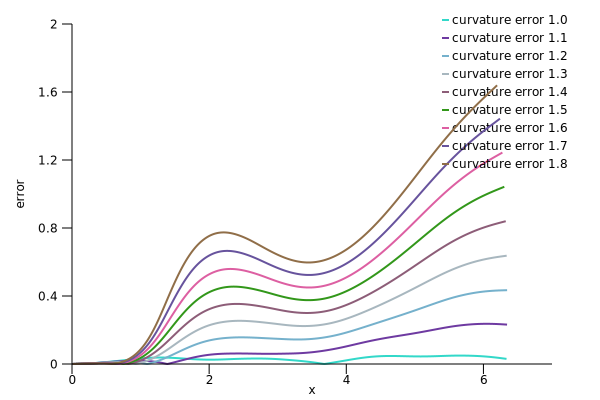
\includegraphics{cos-single-error.pdf}
\caption{单点误差的传递}
\label{fig:cos-single-error}
\end{figure}

图 ~\ref{fig:cos-multiple-error-view} 为曲线上多点分别加入$1.2$曲率数据误差的重建结果。
图 ~\ref{fig:cos-multiple-error} 展示了横坐标$x$变化下分别加入多点曲率误差的的重建误差传递。

可知$s=4.672$处引入曲率误差对重建结果的影响最小,而$s=0.000$处引入对整体曲线影响最大,
但$s=3.820$处引入对后半段曲线的重建结果影响最大,总体来说没什么规律可循。

\begin{figure}[H]
\centering
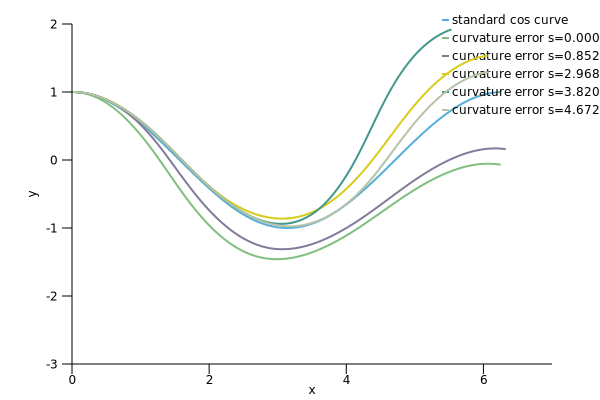
\includegraphics{cos-multiple-error-view.pdf}
\caption{加入多点误差的重建结果}
\label{fig:cos-multiple-error-view}
\end{figure}

\begin{figure}[H]
\centering
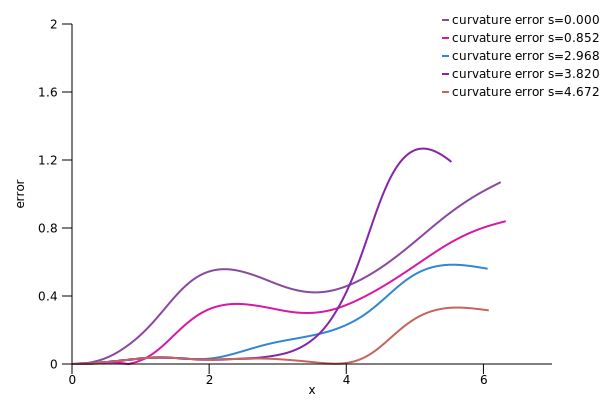
\includegraphics{cos-multiple-error.pdf}
\caption{多点误差的传递}
\label{fig:cos-multiple-error}
\end{figure}


\section{客户端程序实现}

三维渲染采用WebGL渲染引擎和Threejs库,主要功能是根据服务器下推的点列实时渲染管壁或轴线。

WebGL是浏览器上的OpenGL实现,用于在任何兼容的Web浏览器中呈现交互式3D和2D图形\cite{webgl}。
WebGL通过引入一个与OpenGL ES 2.0紧密相符合的API,可以在HTML5 <canvas>元素中使用。

目前支持WebGL的浏览器有:Firefox 4+、Google Chrome 9+、Opera 12+、Safari 5.1+和Internet Explorer 11+;
但是WebGL一些特性也需要用户的硬件设备支持。

WebGL几乎是完全地“跨平台”,使用任何支持WebGL的浏览器打开网页即可完成客户端渲染,而无需下载另外的软件或浏览器插件。

Three.js是一个基于WebGL的3D图形库\cite{threejs},它封装了很多实用的图形组件。

\subsection{轴线渲染}

首先根据下推的点列拟合一条Catmull Rom曲线:

\begin{lstlisting}[language=JavaScript,
   backgroundcolor=\color{lightgray},
   extendedchars=true,
   basicstyle=\footnotesize\ttfamily,
   showstringspaces=false,
   showspaces=false,
   numbers=left,
   numberstyle=\footnotesize,
   numbersep=9pt,
   tabsize=2,
   breaklines=true,
   showtabs=false,
   captionpos=b]

socket.addEventListener('message', event => {
    if (event.data instanceof Blob) {
        event.data.arrayBuffer().then(buffer => {
            let json = inflateRaw(new Uint8Array(buffer), { to: 'string' })
            let data = JSON.parse(json) as Curve
            curve = new THREE.CatmullRomCurve3(data.points.map(
                ({ x, y, z }) => (new Vector3(x, y, z)),
            ))
        }).catch(err => {
            console.log(err)
        })
    }
})
\end{lstlisting}

再定义基础线材质,根据曲线和材质渲染形状并填入缓冲形状:

\begin{lstlisting}[language=JavaScript,
   backgroundcolor=\color{lightgray},
   extendedchars=true,
   basicstyle=\footnotesize\ttfamily,
   showstringspaces=false,
   showspaces=false,
   numbers=left,
   numberstyle=\footnotesize,
   numbersep=9pt,
   tabsize=2,
   breaklines=true,
   showtabs=false,
   captionpos=b]
const material = new THREE.LineBasicMaterial()
const bufGeometry = new THREE.BufferGeometry()
export const object = new THREE.Line(bufGeometry, material)
export const update = () => {
    material.setValues({color: config.color})
    if (curve !== null) {
        bufGeometry.setFromPoints(curve.getPoints(100))
    }
}
\end{lstlisting}

\subsection{管壁渲染}

管壁渲染基于同样的Catmull Rom曲线,但使用网格材质,双边渲染,反光度$100$:

\begin{lstlisting}[language=JavaScript,
   backgroundcolor=\color{lightgray},
   extendedchars=true,
   basicstyle=\footnotesize\ttfamily,
   showstringspaces=false,
   showspaces=false,
   numbers=left,
   numberstyle=\footnotesize,
   numbersep=9pt,
   tabsize=2,
   breaklines=true,
   showtabs=false,
   captionpos=b]
const material = new THREE.MeshPhongMaterial({
    shininess: 100,
    side: THREE.DoubleSide,
})
const bufGeometry = new THREE.BufferGeometry()
export const object = new THREE.Mesh(bufGeometry, material)
export const update = () => {
    material.setValues({color: config.color})
    if (curve !== null) {
        let geometry = new THREE.TubeGeometry(
            curve,
            64,
            0.1,
        )
        bufGeometry.fromGeometry(geometry)
        geometry.dispose()
    }
}
\end{lstlisting}

\subsection{控制器}

主要使用的控制器为轨道控制器,绕原点旋转,启用阻尼:

\begin{lstlisting}[language=JavaScript,
   backgroundcolor=\color{lightgray},
   extendedchars=true,
   basicstyle=\footnotesize\ttfamily,
   showstringspaces=false,
   showspaces=false,
   numbers=left,
   numberstyle=\footnotesize,
   numbersep=9pt,
   tabsize=2,
   breaklines=true,
   showtabs=false,
   captionpos=b]
const orbitControls = new OrbitControls(camera, renderer.domElement)
orbitControls.target = new THREE.Vector3(0, 0, 0)
orbitControls.autoRotate = false
orbitControls.enableDamping = true
orbitControls.dampingFactor = 0.05
\end{lstlisting}

\subsection{环境光}

环境光使用了一个颜色为$\#111111$的全局光和一个颜色为$\#505050$的点光源。

\begin{lstlisting}[language=JavaScript,
   backgroundcolor=\color{lightgray},
   extendedchars=true,
   basicstyle=\footnotesize\ttfamily,
   showstringspaces=false,
   showspaces=false,
   numbers=left,
   numberstyle=\footnotesize,
   numbersep=9pt,
   tabsize=2,
   breaklines=true,
   showtabs=false,
   captionpos=b]
scene.add(new THREE.AmbientLight(0x111111))
let spotLight = new THREE.DirectionalLight(0x505050, 1.5)
spotLight.position.set(0, 1000, 0)
spotLight.castShadow = true
spotLight.shadow.camera.near = 3
spotLight.shadow.camera.far = 10
spotLight.shadow.mapSize.width = 1024
spotLight.shadow.mapSize.height = 1024
scene.add(spotLight)
\end{lstlisting}

\section{软件运行效果}
最终的软件运行效果总体来说很令人满意:运行速度快,稳定60帧渲染;全程TLS加密,安全有保障;
可运行中动态上推、渲染、订阅新的数据源,使用体验极佳。

具体展示见附件二。

\section{总结与展望}
本文总体来说达到了预期目标,使用的也全是当代最先进的技术。
其中WebSocket正支持着成千上万的应用;
TLS保障着整个互联网的安全;
Rust正在为Firefox添砖加瓦;
WebGL定义了下一代的三维渲染程序;
TypeScript是JavaScript社区最受欢迎的转译语言。

从架构方面来说,
渲染任务分离。服务器负责重建,所有的客户端 (浏览器)共享同一份重建数据并渲染。它
大大减少了重建算法的计算压力,仅需一个强有力的服务器完成一次重建,所有的客户端都可以共享重建结果。 
同时,它大大提升了用户的使用体验。在这种架构下,传感器、服务器和客户端即使放置在地球上有互联网覆盖的任意三点,
服务也不会中断。并且终端用户也无需从特定的机器或软件访问服务,而只需要打开任何支持WebGL和TLS
技术的浏览器,即可安全快捷地获得服务。

当然从完成度上来说,这份软件只达到了最小可用的要求,它还需要根据实际需求添加更多的功能以及对现有功能进行调整。
比如添加用户认证系统或者在渲染中更高级的动态分析。

要想构建一个成熟通用的实时三维可视化软件,还有很长的路要走,很多问题有待解决。
